\section{TLS and connection security}

\subsection{Public Key Infrastructure}

In cryptography, a \textbf{digital certificate} or a \textbf{public key
certificate} is an electronic document that attests the validity of an
associated public key. The certificate also contains information that can be
used to identify its owner (i.e., the subject) as well as a trusted third party
responsible for verifying the contents of said certificate (i.e., the issuer).
This latter third party is the crux of digital certificate scheme since all
parties involved must have implicit trust in it.

The issuer is more commonly known as a \textbf{Certificate Authority (CA)}. One
example of a CA is \href{https://letsencrypt.org/}{Let's Encrypt}. This
particular CA was created after Google announced in 2014 that moving forward,
HTTPS support would factor into their search engine result ranking. Let's
Encrypt became available to the public two years later (after a number of
limited, closed tests) and offered the simplest procedure of being issued a
certificate: in order to prove that you were the owner of a domain name, you
needed to run an HTTP server on the standard port 80, at the IP that the domain
name resolved to. On that server, you had to make available a challenge string
that the CA generated for each certificate issuance request. Today, this entire
process has been automated with tools such as
\href{https://certbot.eff.org/instructions}{certbot}.

Although Let's Encrypt contributed to the large-scale adoption of traffic
encryption in the Internet by providing a free and simple certificate issuance
process, note that it offers the lowest level of identity verification. While
most would find this sufficient for the purpose of hosting a web site, larger
organizations such as banks, or businesses engaged in e-commerce require a
more involved vetting process:

\begin{itemize}
    \item \textbf{Domain Validation (DV):} The CA verifies only that the
          applicant controls the domain. The certificate contains information
          about the domain name, but nothing related to the organization that
          owns it. The issuance of these types of certificates is easily
          automated, takes little time (usually minutes) and presents low costs.
          Although perfectly capable of ensuring an encrypted communication
          channel between two parties, little to no trust can be placed in its
          owner. It is very common for phishing web sites to obtain DV
          certificates.

    \item \textbf{Organization Validation (OV):} In addition to domain control,
          the CA also verifies the identity of the organization by means of
          business records proving its legal existence, phone verification, etc.
          The issued certificate will also incorporate the organization's name
          and sometimes address. This type of certificate offers a higher
          level of trust than DV by confirming the legitimacy of the
          organization, but comes at a higher monetary cost and can take hours
          or even days to be issued. OV certificates are mostly recommended for
          small businesses.

    \item \textbf{Extended Validation (EV):} A more rigurous vetting process
          that involves checking domain control, the status of the legal
          organization, its physical address, and sometimes manually verifying
          government records. In this case, the certificate also includes the
          jurisdiction of incorporation. This type of certificate offers
          maximum trust and is most suited for banking sites, government
          portals, large e-commerce applications, etc. Although more costly, it
          is necessary to understand that the issuance fee is far from
          prohibitive, it ranging between \$150-\$600 on average, depending on
          the CA. The issuance process usually takes a few working days.
\end{itemize}

In order for digital certificates to be a practical choice in establishing
secure communication channels and authenticating the peer (usually the server)
a framework for managing and distributing CA certificates is indispensible.
During the early days of the Internet, one such solution was called the
\textbf{Web of Trust}. Under this model, each individual was responsible for
maintaining a \textit{"keychain"} of trusted public keys. Ideally, these keys
would be exchanged in-person. However, this approach was not practical. So,
starting with a small selection of trusted keys, the trusted peers could sign
the public keys of new entities that could then be verified and imported with
different levels of trust. An implementation of these principles dating back to
1991 is  \textbf{Pretty Good Privacy (PGP)} and was used extensively in
encrypting and authenticating emails. The adoption of PGP later lead to the
development of the \textbf{OpenPGP standard} \cite{callas2007rfc} and new
open-source solution such as the \textbf{GNU Privacy Guard (PGP)} being
developed.

Due to scalability issues with this model, another more centralized approach
was proposed. This became known as the \textbf{Public Key Infrastructure (PKI)}
and is now the predominant certificate distribution method used in the Internet.
This paradigm ensures that all operating systems come with a set of CA
certificates already installed. When establishing a connection to a new server
using the \textbf{Transport Layer Security (TLS)} protocol, the server will
provide not only its own certificate, but also the certificate of the CA that
attests its identity, as well as all the other CAs that authenticate one
another (yes, CAs need to be certified by other CAs as well). The top-level CA
has a \textbf{self-signed} certificate and is assumed to be implicitly trusted
by most systems. A company can install its own certificate on employee devices,
thus becoming a root CA in a limited capacity. Real-world examples of root CAs
include Let's Encrypt, DigiCert, Microsoft, etc. The number of root CAs varies
but in 2025 there are approx. 100-150 CAs globally whose root certificates are
are widely trusted by major plaforms (i.e., operating systems and browsers).


\subsection{Transport Layer Security}

Previously we discussed the role of PKIs in the establishment of secure network
connections through TLS. When researching this subject, you may come across an
alternative term, namely \textbf{Secure Socket Layer (SSL)}. In the (very) early
days of the \textbf{World Wide Web (www)}, the most popular browser was NCSA
Mosaic. Although instrumental in popularizing the Wold Wide Web at the time, it
did lack a number of features, such as HTML frames (i.e., the ability to split
a page in different scrollable sections). A contender that would eventually
overtake Mosaic's market share was initially called \textit{Mozilla}, short for
\textit{Mosaic Killer}. Ultimately it would end up being known as Firefox, but
at that time, the creators were forced to change its name to Netscape Navigator
due to legal reasons. In 1995, Netscape relseased SSL 2.0 to ensure
confidentiality, integrity and authentication between the browser and the
server. Although HTTPS today is based on TLS, SSL was the foundation on which
this protocol was originally built. In case you are wondering, there was also a
SSL 1.0 but it was never released to the public due to serious security flaws.
Version 2.0 was not perfect either, implementing weak key exchange algorithms
and not having message integrity checks. In 1996, these problems were addressed
with the help of cryptographer Paul Kocher in the SSL 3.0 release. Later in
1999, as SSL 3.1 was being released, it was agreed that the \textbf{Internet
Engineering Task Force (IETF)} (i.e., the internet standards body that oversees
the development of protocol specifications such as HTTP, TCP, etc.) would take
over the responsibility of maintaining SSL. For political reason, SSL 3.1 was
rebranded into TLS 1.0 and its specification was released in RFC 2246
\cite{dierks1999rfc2246}. The most recent version of TLS is 1.3 and was
published in 2018 as RFC 8446 \cite{rescorla2018rfc}. Although SSL officially
ceased to exist back in 1999, both people and legacy software still refer to TLS
as SSL.

\begin{figure}[h]
    \centering
    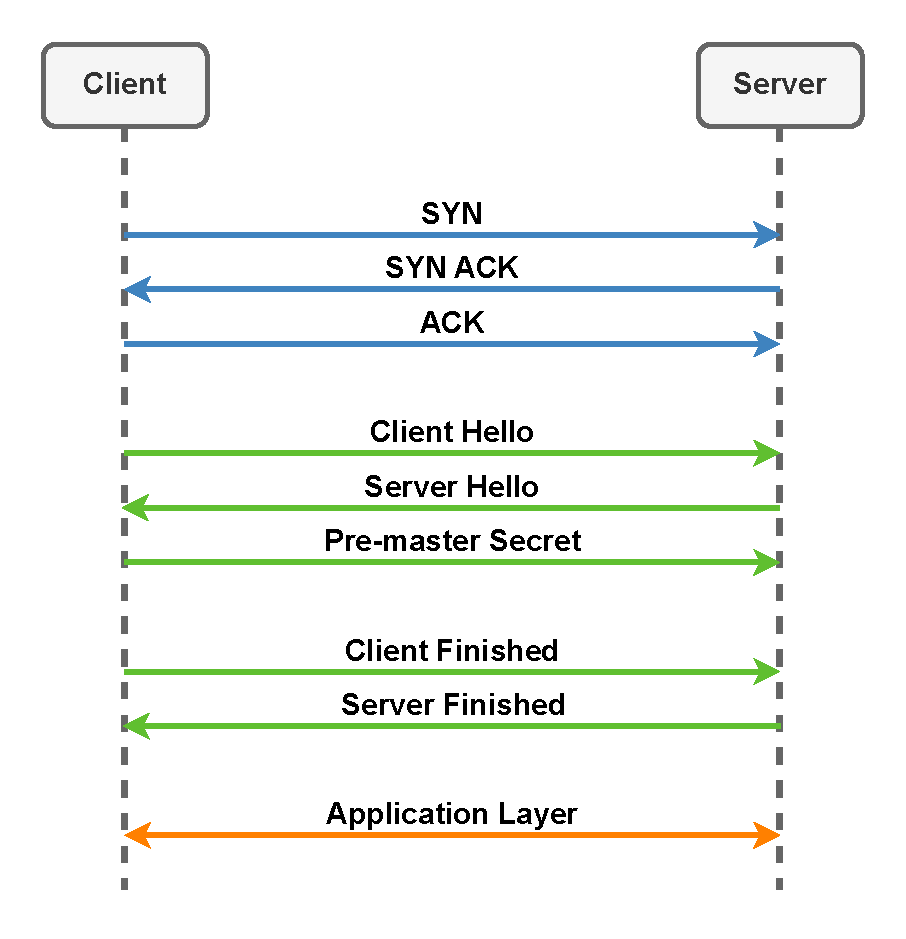
\includegraphics[width=0.9 \textwidth,keepaspectratio]{figures/tls-handshake.pdf}
    \caption{TLS handshake}
    \label{fig:tls-handshake}
\end{figure}

As can be seen in Figure \ref{fig:tls-handshake}, a TLS session starts with a
TCP handshake. Note that using an IP | TCP | TLS stack is most common in the
Internet, but this is not a strict necessity. One could just as well use TLS
over CAN Bus, a serial communication protocol used mostly in automotive local
networks. The only requirement is that the alternative network stack offer TLS
certain guarantees: ordered delivery, error correction, flow control, etc.
Since CAN Bus can offer error correction but now flow control for example, one
must pick and choose the appropriate network protocols. In this case, one
solution would be to construct a CAN | ISO-TP | TLS stack instead. The take-away
here is that TLS is not bound to a specific network stack, in the way that RPC
protocols today are dependent on the TCP/IP stack. Instead, TLS is very flexible
and can be used in almost any situation.

Returning to the figure, we see that both the client and the server exchange
\textit{hello} messages. In these messages, they negociate which version of TLS
will be used moving forward, as well as what collection of cryptographic
algorithms will be employed. This collection is referred to as a
\textit{cyphersuite}. Additionally, the server will send the client its
certificate for validation and can optionally request the client's certificate
for mutual authentication. This is called \textbf{mTLS} and is more commonly
encountered in private, internal networks where for example, each employee is
provided with a work computer with its own certificate that can authenticate
him to a service he wants to access.

After agreeing on all these, the client will send a pre-master secret, encrypted
with the public key from the server's certificate. Both parties will use this
secret material to derive a symmetric key called the \textit{session key}. Here
we remember that asymmetric encryption is a computational intensive operation.
As long as a symmetric key can be exchanged \textit{securely}, it is more
advantageous to use symmetric encryption in high-throughput data exchanges.

Once both the server and client confirm the establishment of the TLS connection,
the application can start the data transfer.
